


The Chang'E-4 mission, initiated in the end of 2018, coincided with a period of solar minimum characterized by a scarcity of \ac{SEP} events. However, as sun stepping into the increase phase of new \ac{SC} and becoming more active than the solar minimum, solar activity has intensified, and consequencely, a growing number of \acs{SEP}, including prolonged-duration and high-intensity one, have been observed to reach the lunar surface and detected by the \ac{LND} on the lunar far-side surface. For example, Guo et al. (2023, in press) recently reported the first \ac{GLE} of \ac{SC} 25, which were concurrently detected by instruments deployed on the Moon, Earth, Mars and also by \ac{SolO} as well as \ac{PSP} [citation of other studies]. It is noteworthy that \ac{LND} was switched on after the initial phase of the event, hence did not cover the whole event. Even so, it still improves our understanding of potential radiaton risk that caused by those extreme \ac{SEP} events on the planetary surface.
In the appendix section of this thesis, a comprehensive list of \ac{SEP} events detected by the \ac{LND} on the lunar far-side surface between 2019 and 2023 is provided, further emphsizing on \ac{LND}'s contribution to the study of \acs{SEP}.


The \ac{SEP} event happened on May 6, 2019 is the first \ac{SEP} event that have ever been detected on the lunar surface, according to our knowledge. 
This \ac{SEP} event is associated with an M-class flare originating from solar active region (AR12470) which is located on the eastern hemisphere and is more than 110 degrees away from the Earth's magnetic footpoint on the solar surface. The remote-sensing observations conducted by the \ac{SOHO}/\ac{LASCO} and \ac{STEREO} revealed the presence of a slow, narrow, and westward moving \ac{CME}. 
Though those \acs{SEP} cause negligible radiation dose due to its weak intensity and lower peak energy, it is still an interesting event and worth studying due to the following two reasons.
The primary objective of this study is to utilize the first \ac{SEP} event observed by \ac{LND} to validate the data products produced during \ac{SEP} occurrences and assess the instrument's performance under such conditions. By cross calibrating the proton measurements between \ac{LND} and other already existed particle instruments at the first lagrange point, specifically the \ac{EPHIN} onboard \ac{SOHO} and \ac{ACE}/\ac{EPAM}, we conclude that \ac{LND} provide reliable solar energetic proton measurement with high time resolution of one minute.
%For sure LND is outside of the mangetosphere, but still that is one of the thing worth to look at. How the SEP propogarting across the magnetosphere and arrive the magnetosphere tails.
Additionally, we aim to investigate the reason of extensive spatial distribution of this \ac{SEP}. Unlike the typical widespread \ac{SEP} events which persist for few days and are accompanied with broad \ac{CME}, the temporal profile of this event and remotesensing observation imply that it is an impulsive event that has good magnetic connections. Several mechanisms could be invovled in the process of the particle traversal across considerable distance in the so-call wide spread \acs{SEP}. 
%Combined the in-site and remote-sensing measurement, we try to found out what kind release and propagation mechanism are involved in this event.

\textit{Short Overview of the publication}
First, we check and analyze the in-situ data from May 3, 2019 to May 8, 2019 in details fron different view points and different detectors. Proton and electron flux, solar wind parameters and local magnetic field measured at L1 point are given.
Though STA had better magnetic connection, the background on the STA is dominated by the pre-existing \ac{SEP}, hence not shown here.
Then we determine the onset time based on the combined data from \ac{LND}, \ac{EPHIN} and \ac{EPAM}. A possion-CUSUM method is applied to tackle the lower statistic measurement. By fitting the velocity dispersion, we derived the release time of the \ac{SEP} event. Besides, the integral spectra of the \ac{SEP} event is also given. In the end of observation section, we analyze the remote-sensing observation including X-ray flux, radio observation \ac{CME} and EUV waves observations.

The key observations of the publication are:
\begin{itemize}
    \item \ac{LND} has consistent measurements as other L1 instruments during the first \ac{SEP} events, including the consistent onset time and spectra.
    \item Proton electron profile show clearly velocity dispersion and beam like structure. The release time of electron is an hour earlier than the proton.
    \item The magnetic footpoint of Earth is about 113$^\circ$ away the flare location. The accompanied \ac{CME} is slow and narrow. We found no evidence of EUV arrival at the magnetic footpoint of Earth. 
    \item The more than 100 degree longitudianl seperation are hard to explain in a impulsive \ac{SEP} event. Possible reasons include the expanding coronal shock, irregular magnetic field, and random walk of magnetic field line, or the mixture of above three. Besides, the release mechanism of electron and proton might be different due to their distinct behaviors.
\end{itemize}

The following article is reproduced from \textcite{Xu2020ApJ} by permission of the AAS:\\

\noindent\pubcite{Xu2020ApJ}\\
\strut\hfill Own contribution: 80\%

\newpage
\newcounter{includepdfpageAPJLTwenty}

\addtocounter{section}{1}
\setcounter{section}{1} 
% \phantomsection
% \addcontentsline{toc}{section}{\arabic{chapter}.\arabic{section} First Solar Energetic Particles Measured on the Lunar Far-side(Publication ApJ Letter 2020)}
%
\phantomsection
\addcontentsline{toc}{section}{\arabic{chapter}.\arabic{section} Introduction}
\label{sec:paper_xu2020}
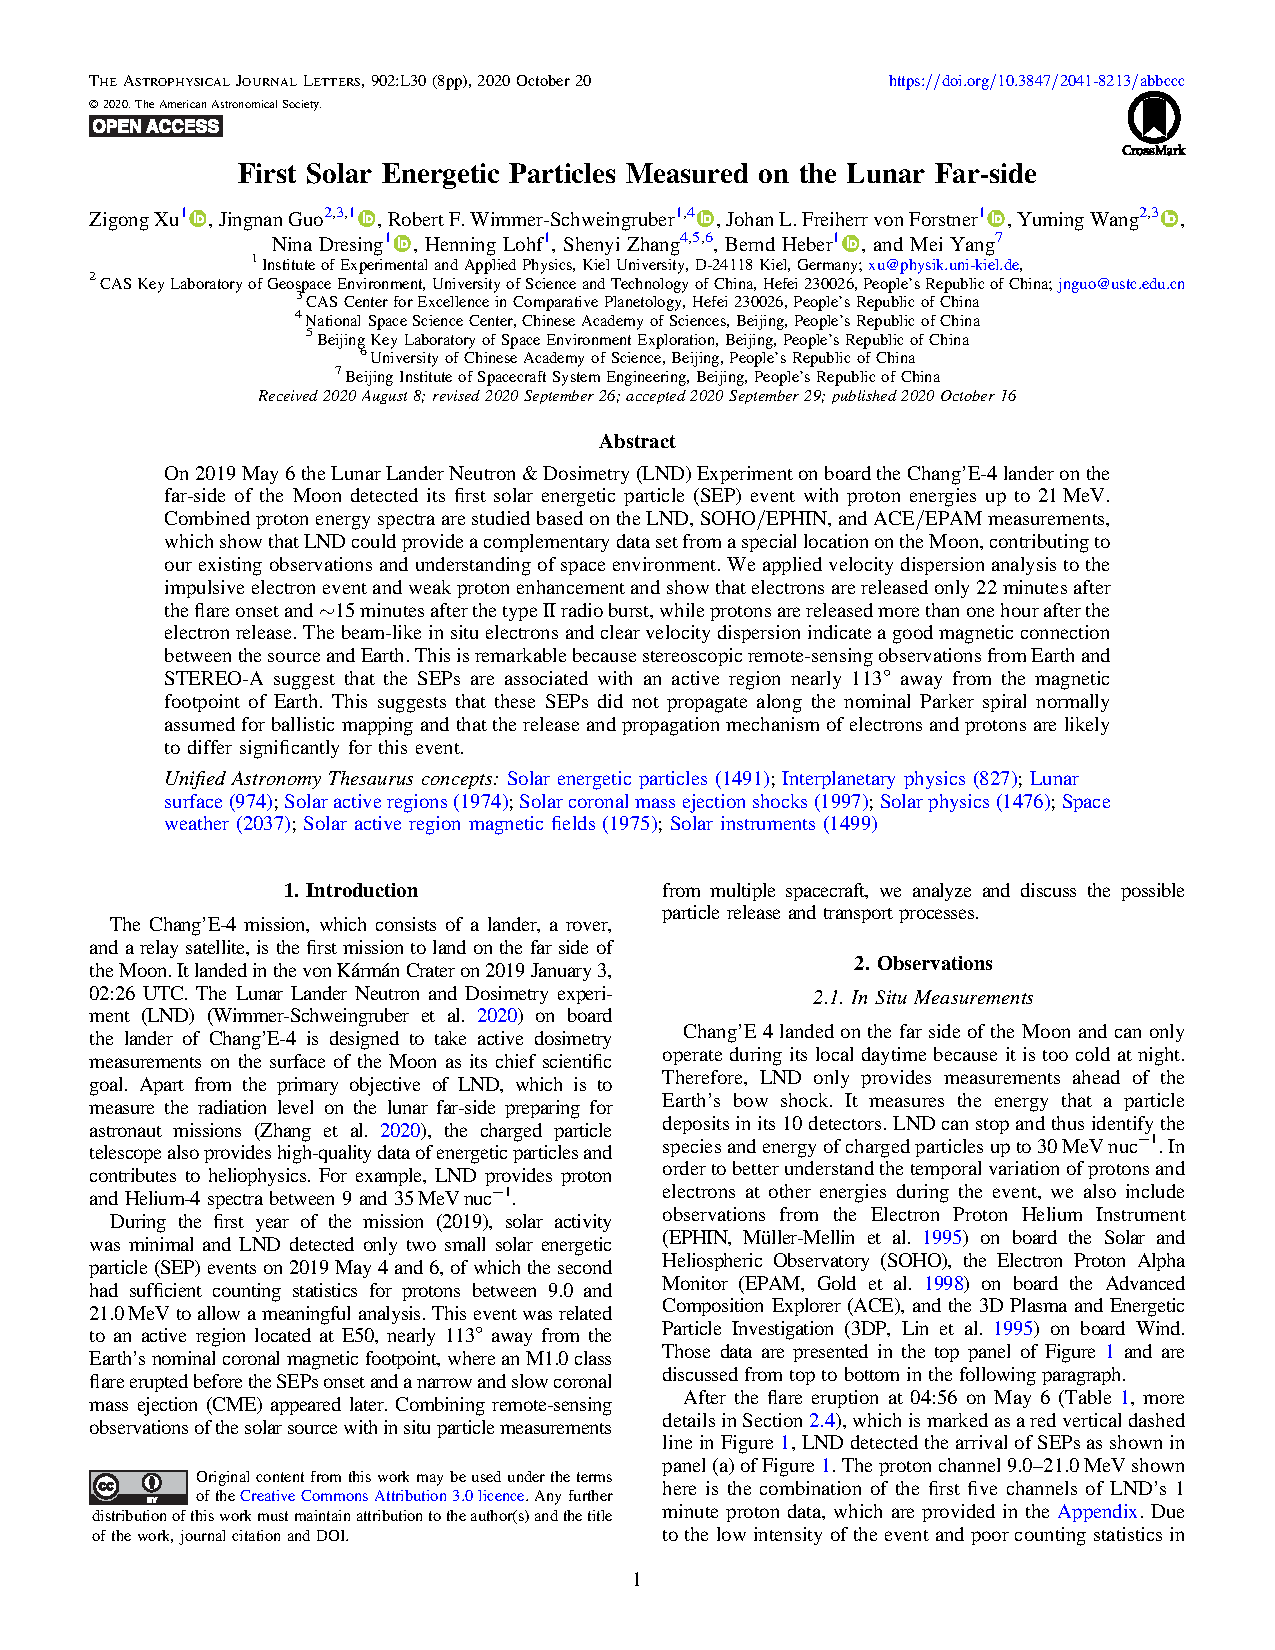
\includepdf[pages={1}, link, linkname=paper_xu2020, scale=.9, pagecommand={\refstepcounter{includepdfpageAPJLTwenty}\label{paper_xu2020.\theincludepdfpageAPJLTwenty}}]{publications/Xu_et_al_2020_ApJL.pdf}
%
\addtocounter{section}{1} 
\phantomsection
\addcontentsline{toc}{section}{\arabic{chapter}.\arabic{section} Observations}
\includepdf[pages={2-4}, link, linkname=paper_xu2020, scale=.9, pagecommand={\refstepcounter{includepdfpageAPJLTwenty}\label{paper_xu2020.\theincludepdfpageAPJLTwenty}}]{publications/Xu_et_al_2020_ApJL.pdf}
%
\addtocounter{section}{1} 
\phantomsection
\addcontentsline{toc}{section}{\arabic{chapter}.\arabic{section} Summary and Discussion}
\includepdf[pages={5-6}, link, linkname=paper_xu2020, scale=.9, pagecommand={\refstepcounter{includepdfpageAPJLTwenty}\label{paper_xu2020.\theincludepdfpageAPJLTwenty}}]{publications/Xu_et_al_2020_ApJL.pdf}
%
\addtocounter{section}{1} 
\phantomsection
\addcontentsline{toc}{section}{\arabic{chapter}.\arabic{section} Appendix}
\includepdf[pages={7}, link, linkname=paper_xu2020, scale=.9, pagecommand={\refstepcounter{includepdfpageAPJLTwenty}\label{paper_xu2020.\theincludepdfpageAPJLTwenty}}]{publications/Xu_et_al_2020_ApJL.pdf}
%
\addtocounter{section}{1} 
\phantomsection
\addcontentsline{toc}{section}{\arabic{chapter}.\arabic{section} References}
\includepdf[pages={8}, link, linkname=paper_xu2020, scale=.9, pagecommand={\refstepcounter{includepdfpageAPJLTwenty}\label{paper_xu2020.\theincludepdfpageAPJLTwenty}}]{publications/Xu_et_al_2020_ApJL.pdf}
